
\section{Quadrature}

\label{sec:quadrature}

Numerical quadrature refers to numerical integration in one dimension.

\begin{definition}[$n$-point Quadrature rule]
    An $m$-point quadrature rule on $[a,b]$, $n \in \mathbb{N}$ is defined as \cite{hiptmair_numerical_2023}
    \begin{align}
        \int_a^b f(t) \ \mathrm{d}t \approx \sum_{j=1}^n w_j \, f(x_j),
    \end{align}
    where $w_j \in \R$ are the \emph{quadrature weights} and $x_j \in [a, b]$ are the \emph{quadrature nodes}.
\end{definition}

A quadrature rule defines a way to approximate a definite integral of a function using a weighted sum of the values of the function at specific points, also defined by the quadrature rule, called the quadrature nodes or points.
Quadrature rules have a fixed, total number of points $n$ on which they evaluate the function. For each point $j$ of the $n$ points, the rule also defines a weight for the weighted sum.

In this work, numerical quadrature is required to approximate the integral in the computation of the element matrix of the cell-oriented assembly algorithm (see section \ref{sec:assembly}).

There are many different quadrature rules, with different properties.
To talk about the accuracy of quadrature rules, one can use the \emph{degree of exactness} of a quadrature rule, often abbreviated as just the \emph{degree} of a quadrature rule.

\begin{definition}[Degree of a quadrature rule]
    A quadrature rule has \emph{degree (of exactness)} $m$ if $m$ is the maximal degree of the polynomials
    for which the quadrature rule is guaranteed to be exact \cite[Def.~7.4.1.1]{hiptmair_numerical_2020}.
\end{definition}

This means the quadrature rule of degree $m$ provides exact solutions (instead of just approximations)
for all polynomial functions $f$ with degree lower or equal to $m$. For non-polynomial functions or
polynomials with a degree greater than $m$, it only provides an approximation.

In literature, it is often the order that is used to compare different quadrature rules.

\begin{definition}[Order of a quadrature rule]
    The order $p$ of a quadrature rule of degree $m$ is: \cite[Def.~7.4.1.1]{hiptmair_numerical_2020}
    \begin{align}
        p = m + 1.
    \end{align}
\end{definition}

Some examples of the degrees, and orders, of quadrature rules are:
\begin{itemize}
    \item Midpoint (Rectangle) rule: Degree 1 (Order 2).
    \item Trapezoidal rule: Degree 1 (Order 2).
    \item Simpson rule (3-point): Degree 3 (Order 4).
    \item $n$-point Gaussian quadrature rule: Degree $2n - 1$ (Order $2n$).
\end{itemize}

\subsection{Gaussian-Quadrature}

\begin{definition}[$n$-point Gaussian quadrature rule]
    An $n$-point Gaussian quadrature rule is a quadrature rule that yields exact results for polynomials of degree $2n - 1$ or less.
    It is defined on $[-1, 1]$ as:
    \begin{align}
        \int_{-1}^1 f(x) \ dx \approx \sum_{i=1}^n w_i f(x_i).
    \end{align}
    Therefore, by definition, a Gaussian quadrature rule has degree $2n - 1$ and order $2n$.
\end{definition}

The weights $w_j \in \R, \ j=1, ..., n$ of an $n$-point quadrature rule on $[-1, 1]$ are given by
\cite[Thm.~7.4.1.6]{hiptmair_numerical_2020}:
\begin{align}
    w_j = \int_{-1}^1 L_{j-1}(t) \ dt, \quad j=1, ..., n,
    \label{eq:quad_weights}
\end{align}
where $L_k, \ k = 0, ..., n-1$ is the $k$-th Lagrange polynomial associated with the ordered
set of quadrature nodes $\{ x_1, ..., x_n \}$.

\subsubsection{Gauss-Legendre Quadrature}

The simplest example of a Gaussian quadrature rule is the Gauss-Legendre quadrature rule,
which uses the Legendre polynomials

\begin{definition}[Legendre Polynimial]
    The $n$-th \emph{Legendre polynomial} $P_n$ is defined by \cite[Def.~7.4.2.16]{hiptmair_numerical_2020}:
    \begin{align}
        \int_{-1}^1 P_n(t) q(t) \ dt = 0 \quad \forall q \in \mathcal{P}_{n-1},
    \end{align}
    where $\mathcal{P}_{n-1}$ is the set of polynomials of degree smaller or equal to $n - 1$.

\end{definition}

\begin{definition}[$n$-point Gauss-Legendre Quadrature]
    A $n$-point Gauss-Legendre quadrature rule has the nodes at the zeros (roots) of the $n$-th Legendre polynomial.
    The weights are chosen according to equation \ref{eq:quad_weights}.
\end{definition}


\begin{table}[H]
    \centering
    \renewcommand{\arraystretch}{1.1}
    \small
    \begin{tabularx}{9cm}{>{$}l<{$}| >{$}l<{$}| >{$}l<{$}}
        n & \text{Points} \ x_i         & \text{Weights} \ w_i      \\ \hline
        1 & x_1 = 0                     & w_1 = 2                   \\ \hline
        2 & x_1 = -0.57735026918962...  & w_1 = 1                   \\
          & x_2 = 0.57735026918962...   & w_2 = 1                   \\ \hline
        3 & x_1 = -0.77459666924148...  & w_1 = 0.88888888888888... \\
          & x_2 = 0                     & w_2 = 0.55555555555555... \\
          & x_3 = 0.77459666924148...   & w_3 = 0.88888888888888... \\ \hline
        4 & x_1 = -0.86113631159405...  & w_1 = 0.34785484513745... \\
          & x_2 =  -0.33998104358485... & w_2 = 0.65214515486254... \\
          & x_3 =  0.33998104358485...  & w_3 = 0.65214515486254... \\
          & x_4 =  0.86113631159405...  & w_4 = 0.34785484513745... \\ \hline
        5 & x_1 = -0.90617984593866...  & w_1 = 0.23692688505618... \\
          & x_2 = -0.53846931010568...  & w_2 = 0.47862867049936... \\
          & x_3 = 0                     & w_3 = 0.56888888888888... \\
          & x_4 = 0.53846931010568...   & w_4 = 0.47862867049936... \\
          & x_5 = 0.90617984593866...   & w_5 = 0.23692688505618... \\ \hline
        6 & x_1 = -0.93246951420315...  & w_1 = 0.17132449237917... \\
          & x_2 = -0.66120938646626...  & w_2 = 0.36076157304813... \\
          & x_3 = -0.23861918608319...  & w_3 = 0.46791393457269... \\
          & x_4 = 0.23861918608319...   & w_4 = 0.46791393457269... \\
          & x_5 = 0.66120938646626...   & w_5 = 0.36076157304813... \\
          & x_6 = 0.93246951420315...   & w_6 = 0.17132449237917... \\ \hline
        7 & x_1 = -0.94910791234275...  & w_1 = 0.12948496616887... \\
          & x_2 = -0.74153118559939...  & w_2 = 0.27970539148927... \\
          & x_3 = -0.40584515137739...  & w_3 = 0.38183005050511... \\
          & x_4 = 0                     & w_4 = 0.41795918367346    \\
          & x_5 = 0.40584515137739...   & w_5 = 0.38183005050511... \\
          & x_6 = 0.74153118559939...   & w_6 = 0.27970539148927... \\
          & x_7 = 0.94910791234275...   & w_7 = 0.12948496616887...
    \end{tabularx}
    \caption{Table with Gauss-Legendre quadrature nodes and weights for one to seven points \cite{lowan_table_1942}.}
    \label{table:gauss_legendre}
\end{table}

\pagebreak

\subsection{Gauss-Jacobi Quadrature}

If the function to integrate $f(x), \ f: \R \mapsto [-1, 1]$ has endpoint singularities,
the integrand can be rewritten as $f(x) = (1-x)^\alpha(1+x)^\beta g(x)$,
where $g$ is just the integrable function without the endpoint singularities at $\{-1, 1\}$.
This is known as the Gauss-Jacobi quadrature rule.

\begin{definition}[$n$-point Gauss-Jacobi quadrature rule]
    \begin{align}
        \int_{-1}^1 f(x) \ dx = \int_{-1}^1 (1 - x)^\alpha(1 + x)^\beta g(x) \ dx \approx \sum_{i=1}^n w_i g(x_i),
    \end{align}
    with $\alpha, \ \beta \geq -1$.
\end{definition}

It is important to note that the Gauss-Legendre quadrature is a special case of the Gauss-Jacobi quadrature with $\alpha = \beta = 0$.
Some other special cases of the Gauss-Jacobi quadrature are the Chebyshev-Gauss quadrature of the first kind ($\alpha = \beta = -\frac{1}{2}$),
Chebyshev-Gauss quadrature of the second kind ($\alpha = \beta = \frac{1}{2}$) and Gauss-Gegenbauer quadrature ($\alpha = \beta$).

The Jacobi polynomials, like the Legendre polynomials, are orthogonal polynomials and are defined through a recurrence relation.


\subsubsection*{Algorithm}

To compute the Gauss-Jacobi quadrature nodes, the implementations of deal.II \cite{bangerth_dealiigeneral-purpose_2007},
GSL \cite{gough_gnu_2009}, and LehrFEM++ \cite{craffael_lehrfem_2023} were analyzed.
All of the mentioned libraries use an iterative algorithm to compute the zeros of the polynomials
with the recurrence relation using Newton's method \cite[Chapter~8.5]{hiptmair_numerical_2020}.

The implemented algorithm is mostly based on the implementation from LehrFEM++ \cite{craffael_lehrfem_2023},
since it is best suited our requirements.
For Newton's method, the implementation remained the same as in LehrFEM++.

The steps in the algorithm are:
\begin{enumerate}
    \item Iterate over the number of quadrature points to compute (roots of Gauss-Jacobi polynomial).
    \item For each point, make an initial (educated) guess.
    \item Apply Newton's method on the initial guess to find the root.
    \item Compute the weight corresponding to the point using the root.
\end{enumerate}

The implemented algorithm (see Code \ref{alg:gauss_jac}) also provides the possibility to use different initial guesses.
LehrFEM++ \cite{craffael_lehrfem_2023} uses some custom initial guesses compared to deal.II \cite{bangerth_dealiigeneral-purpose_2007},
which uses the Chebychev nodes for initial guesses.

\begin{Code}
    \small
    \begin{minted}{cpp}
// Compute the root of the Jacobi polynomial
for (std::size_t i = 0; i < NumNodes1D; ++i) {
    // initial guess depending on which root we are computing
    if (initial_guess_type == InitialGuessType::LehrFEM) {
        z = this->getLehrFEMInitialGuess(i, integration_nodes);
    } else if (initial_guess_type == InitialGuessType::Chebyshev) {
        z = -this->getChebyshevNodes(i);
    } else {
        throw std::runtime_error("Unknown initial guess type");
    }

    std::size_t its = 1;
    do {
        // refinement by Newton's method (from LehrFEM++)
        temp = 2.0 + alfbet;

        p1 = (alpha - beta + temp * z) / 2.0;
        p2 = 1.0;
        for (std::size_t j = 2; j <= NumNodes1D; ++j) {
            p3   = p2;
            p2   = p1;
            temp = 2 * j + alfbet;
            a    = 2 * j * (j + alfbet) * (temp - 2.0);
            b    = (temp - 1.0) * (alpha * alpha - beta * beta + temp * (temp - 2.0) * z);
            c    = 2.0 * (j - 1 + alpha) * (j - 1 + beta) * temp;
            p1   = (b * p2 - c * p3) / a;
        }
        pp = (NumNodes1D * (alpha - beta - temp * z) * p1
                + 2.0 * (NumNodes1D + alpha) * (NumNodes1D + beta) * p2)
                / (temp * (1.0 - z * z));

        z1 = z;
        z  = z1 - p1 / pp;  // Newtons Formula

        if (its > this->min_newton_iterations_m && Kokkos::abs(z - z1) <= tolerance) {
            break;
        }
        ++its;
    } while (its <= this->max_newton_iterations_m);

    integration_nodes[i] = z;

    // Compute the weight of the Gauss-Jacobi quadrature
    weights[i] =
        Kokkos::exp(Kokkos::lgamma(alpha + NumNodes1D) + Kokkos::lgamma(beta + NumNodes1D)
                    - Kokkos::lgamma(NumNodes1D + 1.)
                    - Kokkos::lgamma(static_cast<double>(NumNodes1D) + alfbet + 1.0))
        * temp * Kokkos::pow(2.0, alfbet) / (pp * p2);
}
    \end{minted}
    \caption{Abbreviated Algorithm for the computation of the Gauss-Jacobi quadrature nodes and weights.}
    \label{alg:gauss_jac}
\end{Code}


\subsection{Tensor-product Quadrature}

In this chapter, up to now, only one-dimensional quadrature was considered.
However, in this framework, the assembly functions use the quadrature nodes on the reference elements,
which have the same dimension as the mesh that is used.

The reference elements are $n$-cuboids and the quadrature nodes follow the vertices of a tensor-product mesh.

\begin{figure}[h]
    \centering
    \resizebox{0.4\textwidth}{!}{%
        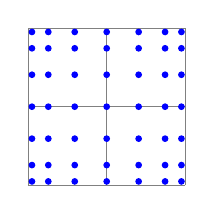
\begin{tikzpicture}
            \draw[step=1cm,gray,very thin] (-1,-1) grid (1,1);
            \foreach \x in {-.94910791234275,-.74153118559939,-.40584515137739,0,.40584515137739,.74153118559939,.94910791234275} {
                    \foreach \y in {-.94910791234275,-.74153118559939,-.40584515137739,0,.40584515137739,.74153118559939,.94910791234275} {
                            \draw[blue,fill=blue] (\x,\y) circle (1pt);
                        }
                }
        \end{tikzpicture}
    }
    \caption{2D Tensor-product of 7-point Gauss-Legendre quadrature nodes on the unit-square.}
    \label{fig:tensor_prod}
\end{figure}
